
%%% Local Variables: 
%%% mode: latex
%%% TeX-master: t
%%% End: 

\chapter{资源管理可编程体系结构PARD}
\label{chap:pardarch}

本章介绍PARD体系结构的基本架构,
并通过管理员视角介绍PARD体系结构的关键特性,包括:
实现全硬件支持的虚拟化、性能监控与反馈、以及可编程的资源管理机制。
最后讨论了如何在现有体系结构中扩展以支持PARD的这些关键特性。

\section{PARD体系结构}

PARD是在传统服务器体系结构的基础上进行功能扩展,
实现可管理的硬件资源共享与区分化服务的计算机体系结构实现。
可以从用户、管理员和体系结构三个视角理解PARD体系结构(图\ref{fig:pard-views}):
从用户的视角,PARD是一个可以划分为多个子机器的计算机,每个子机器可以运行独立的操作系统,
不同用户的子机器之间不会存在干扰,用户可根据自己的需求对资源的使用情况进行约定,
如Cache占用、访存带宽等,对子机器的执行性能可预测;
从管理员的视角,PARD是一台具有硬件资源细粒度管理能力的服务器,
通过服务器上配置的资源管理模块(Platform Resource Manager,PRM),
可以监控每个用户对不同硬件资源的使用情况,并可根据需求对资源使用情况进行调整;
从体系结构的视角,PARD将网络的概念引入到计算机体系结构中,
在体系结构内实现了应用区分,为共享硬件部件增加可编程能力,并实现计算机内统一的资源管理。

\begin{figure}[htb]
  \centering
  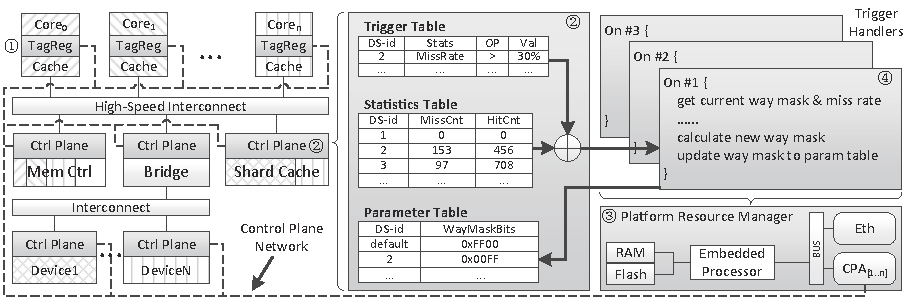
\includegraphics{arch/pard-arch-detail.pdf}
  \caption{PARD体系结构}
  \label{fig:pard-views}
\end{figure}

在多应用混合这种共享场景中,隔离性和可管理性是服务器体系结构设计时需要考虑的重要问题。
\textbf{隔离性}是指要让运行在共享环境中的应用无法感知到其它应用的存在,
就像它正在运行在独占的计算机中一样,这其中包含两个层次的概念:
一是资源隔离,即应用独占分配给它的资源;
二是性能隔离,使得应用的性能不会被其它应用所干扰。
现有的软件方案(如多进程、容器、虚拟化)或硬件方案(如LPAR、Logic Domain)
可以很容易实现不同级别的资源隔离,但它们都无法完全实现性能隔离。
首先,在操作系统或虚拟化的软件栈的各个层次中都存在不同程度的共享,
这些共享点在一些特定的场景会产生干扰;
而即使是硬件隔离方案,虽然消除了软件层次的干扰,但在共享硬件资源上的干扰依然存在。
硬件层次的隔离没有发挥应有的效果主要是由于目前的体系结构中并不能识别不同的应用。
\textbf{可管理性}是能够对应用占用的资源进行监控与管理。
由于不同的应用或应用运行的不同阶段,其对资源的需求是不同且不断变化的,
如何获取应用资源需求的变化,以及如何根据这些变化对资源的分配进行调整。

PARD选择了硬件隔离方案,为用户提供逻辑域的抽象以实现资源隔离,
通过使用标签的方式将服务器划分为不同的地址空间,以实现性能隔离;
在各个硬件部件上增加了控制平面与可编程可能,实现共享资源管理;
通过节点内全局的资源管理,实现资源按需分配与动态调整。


% 关键技术点
\textbf{标签化地址空间}\ 传统计算机架构使用单一地址空间,虽然虚拟内存与扩展页表机制
为不同的应用或虚拟机分配独立的逻辑地址空间,但它们还是共享一个物理地址空间。
这种单一地址空间的设计,使得共享的硬件部件不能识别出来自不同应用的请求,造成

传统服务器中共享的硬件资源主要包括处理器、Cache、内存和I/O等,
在当前数据中心多应用混合的场景下,现有体系结构实现(如x86、ARM等)无法区分不同的应用,
使得计算机中的硬件资源正在被无管理的共享使用,应用之间由于共享产生干扰,
严重影响应用的性能。

\textbf{可管理的硬件资源共享}\ 控制平面,提供统一的编程接口;
数据平面,实现功能可编程;
集成标签化地址空间,实现区分化服务;
提供资源监控与配置的功能,实现硬件资源的可管理。

\textbf{资源按需分配}\ 集中式的资源监控,资源全局调节,Trigger=>Action的反馈调节机制。


\section{PARD示例:用户视图}

本节将以一种虚拟化场景介绍如何利用PARD实现多应用共享硬件,并保证关键应用的服务质量。
本节所述的场景如图\ref{fig:pard-cloud}所示,其中涉及两种角色:
(1)用户,需要使用PARD服务器部署应用,而应用分为延迟敏感型应用与批处理型应用两类;
(1)管理员,管理硬件资源,为用户分配虚拟机以运行应用,同时监控应用性能并对系统进行调整。
在真实的环境中,用户与管理员并不会直接操作服务器本身,而是通过如mesos、OpenStack等集群管理系统使用服务器资源。
这里为了简化描述,将集群管理系统这一层移除,让用户与管理员直接操作服务器。

关键功能+使用方法+流程示意

\begin{figure}[htb]
  \centering
  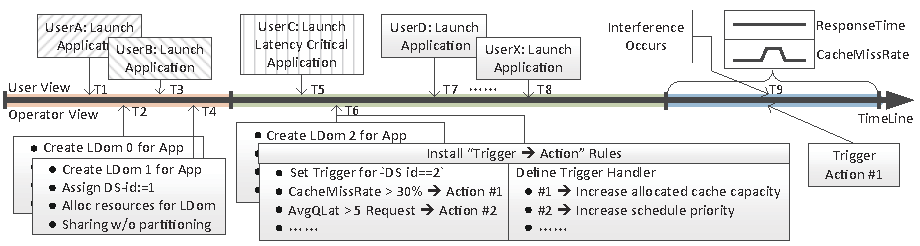
\includegraphics{arch/pard-example.pdf}
  \caption{PARD示例}
  \label{fig:pard-example}
\end{figure}

\subsection{虚拟机创建与关闭}

\subsection{性能监控与反馈}

\subsection{资源调整}

\section{体系结构的可行性}

在X86或ARM上实现该架构

%如何在一个ARM中实现PARD功能

如上节所述,PARD并不是一个完全全新的体系结构,而是对现有体系结构的扩展。
为了说明如何将PARD扩展到一个现有的体系结构中,本节首先构建了一台虚拟计算机,
我们将其命名为XXXX,如图\ref{fig:XXX-computer}所示。
XXX包含两路4核的处理器,每个处理器核拥有独立的一级缓存L1-I和L1-D,
每个Socket的四个处理器核共享一个16路2MB的二级缓存;
两个Socket拥有自己的内存控制器,同时使用MESI目录协议实现NUMA内存访问;
XXX的I/O子系统包含SATA控制器和两个以太网卡,通过IOH芯片与两个处理器相连。
XXX的结构可以很好的匹配到目前流行体系结构中(如X86或ARM)。

\subsection{Computer as a Network => PARD}

\subsection{像SDN一样集中式的管理计算机}

\section{PARD与SDN}

在第\ref{chap:intro}章中我们提出
同时,计算机内部也可以被看做一个网络,如图\ref{fig:computer-as-a-network}所示,
CPU核、共享缓存、内存控制器、I/O设备等可以被看做是网络节点;除了处理请求以外,
这些“网络节点”与网络中的路由器/交换机具有相似的请求转发功能;
而它们之间也通过包进行通信,如:片内通信使用NoC包,片间通信的QPI/HT包,
以及I/O部分使用的PCI-E包。
将网络领域的区分化服务和软件定义网络的思想应用到计算机内部的网络,
用以解决数据中心当前面临的资源利用率与应用服务质量矛盾,是本文的主要研究思路与动机。

与在网络中部署SDN相比,在计算机体系结构“网络”中部署SDN会面临以下三个挑战:

首先,在整个网络栈中EndPoint是唯一的请求来源,因此SDN可以很容易的将标签机制实现在网络栈中;
与之相对的,在计算机体系结构中存在大量的硬件部件都能够发送请求,而这些请求类型又不尽相同,
因此在这样的环境下如何为请求打上标签是一个很大的挑战。

其次,在网络中所有的交换机都执行相同的存储/转发(store-and-forward)操作,但在计算机内部
不同的部件都有不同的功能,而不只是简单的存储/转发,如何为这些不同类型的部件(如末级缓存控制器、
内存控制器、I/O设备等)设计统一的控制面结构是另一个挑战。

最后,在网络交换机中已经包含了一个firmware固件用于访问和配置交换机的控制面,但计算机中却缺少
这样的firmware。现有的IPMI只被用来做有限的监控与管理功能,如对温度、风扇转速和电源控制。
因此,需要在计算机内部提供一种这样的部件实现与其它众多的控制面的通信与管理,并提供一个灵活的
编程接口对这些控制面进行操作。


\begin{figure}[tbh]
  \centering
  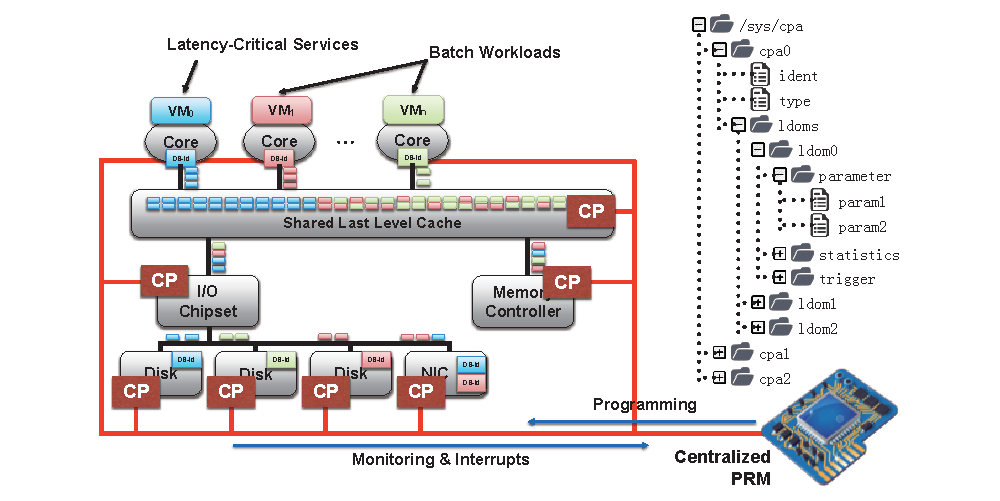
\includegraphics{arch/pard-arch-outline.pdf}
  \caption[PARD体系结构概况]{PARD体系结构概况}
  \label{fig:pard-arch-outline}
\end{figure}

\begin{figure}[tbh]
  \centering
  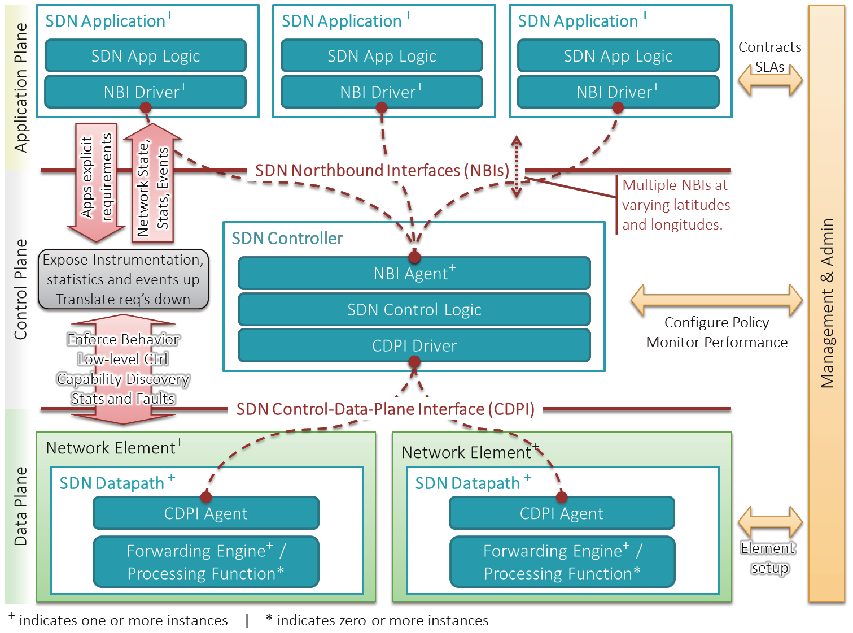
\includegraphics{arch/sdn-arch.pdf}
  \caption{软件定义网络SDN架构}
  \label{fig:pard-arch-outline}
\end{figure}

\section{小结}
